\section{DenseNetチューニング後のモデル図}

\begin{figure}[htbp]
    \centering
    \subfloat[][DenseNet121- 分類器拡張なし (モデル1)]{
        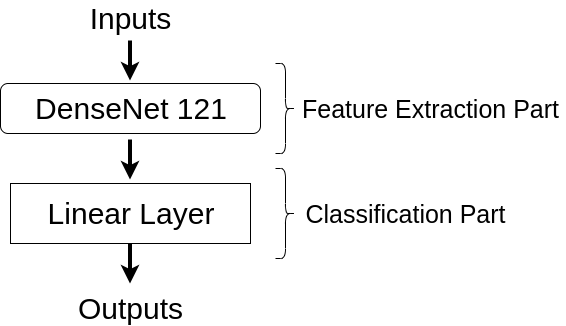
\includegraphics[width=65mm]{./fig/densenet121.png}
        \label{fig:model11}
    } \quad
    \subfloat[][DenseNet121- 分類器拡張あり (モデル2)]{
        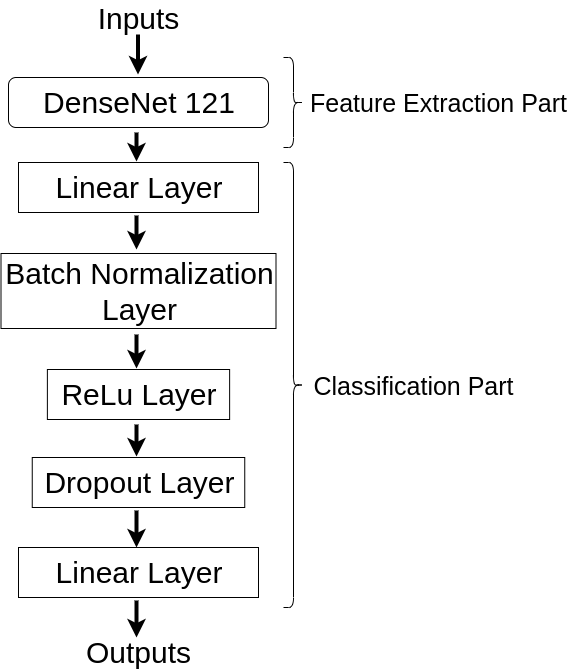
\includegraphics[width=65mm]{./fig/densenet121_e.png}
        \label{fig:model12}
    }
    \caption{DenseNet121チューニング後のモデル図}
\end{figure}

\begin{figure}[htbp]
    \centering
    \subfloat[][DenseNet161- 分類器拡張なし (モデル3)]{
        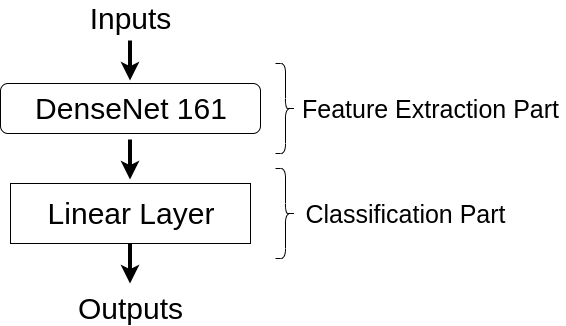
\includegraphics[width=65mm]{./fig/densenet161.png}
        \label{fig:model13}
    } \quad
    \subfloat[][DenseNet161- 分類器拡張あり (モデル4)]{
        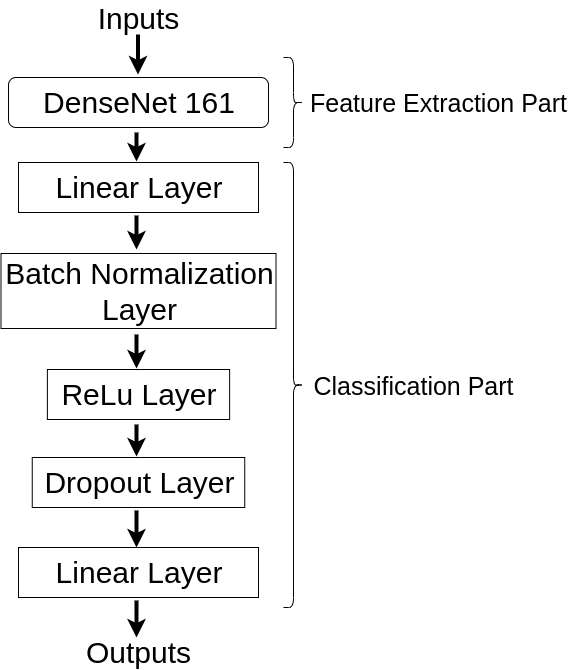
\includegraphics[width=65mm]{./fig/densenet161_e.png}
        \label{fig:model14}
    }
    \caption{DenseNet161チューニング後のモデル図}
\end{figure}

\vspace{3cm}

\section{3D-ResNetチューニング後のモデル図}
\begin{figure}[htbp]
    \centering
    \subfloat[][3D-ResNet-AveragePool- 分類器拡張なし\\ (モデル1)]{
        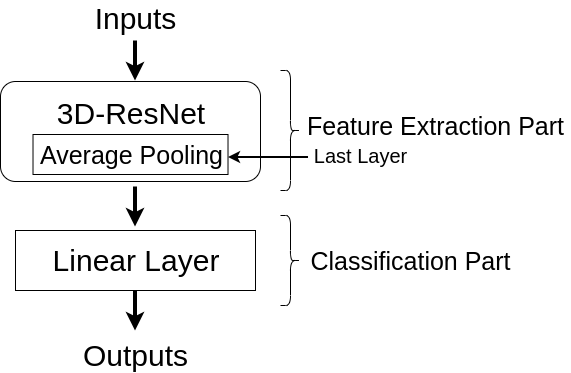
\includegraphics[width=65mm]{./fig/resnet3d.png}
        \label{fig:model21}
    } \quad
    \subfloat[][3D-ResNet-AveragePool- 分類器拡張あり\\ (モデル2)]{
        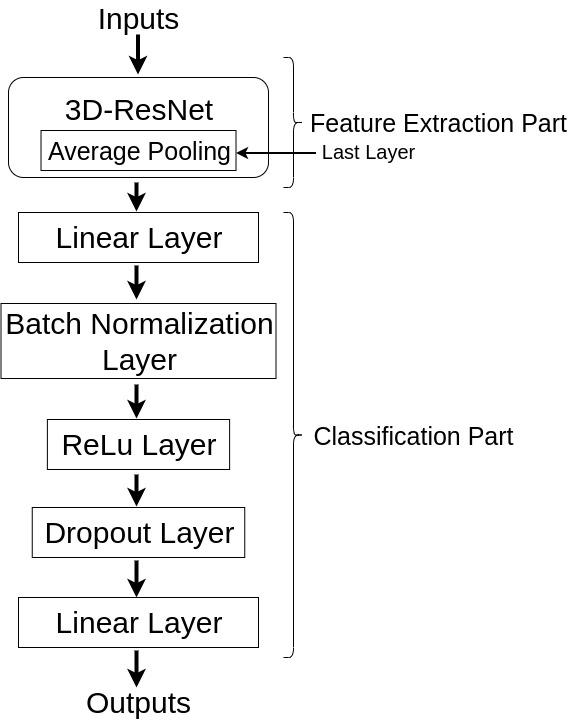
\includegraphics[width=65mm]{./fig/resnet3d_e.png}
        \label{fig:model22}
    }
\end{figure}

\begin{figure}[htbp]
    \centering
    \ContinuedFloat
    \subfloat[][3D-ResNet-MaxPool- 分類器拡張なし\\ (モデル3)]{
        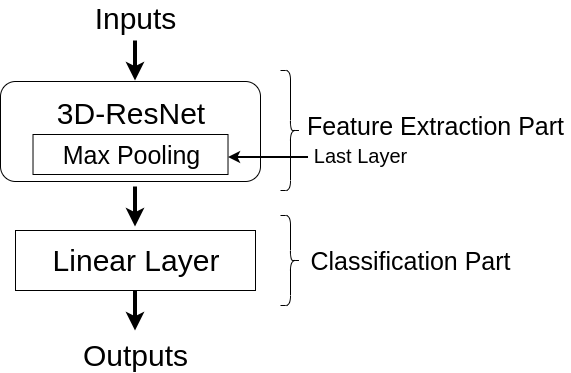
\includegraphics[width=65mm]{./fig/resnet3d_m.png}
        \label{fig:model23}
    } \quad
    \subfloat[][3D-ResNet-MaxPool- 分類器拡張あり\\ (モデル4)]{
        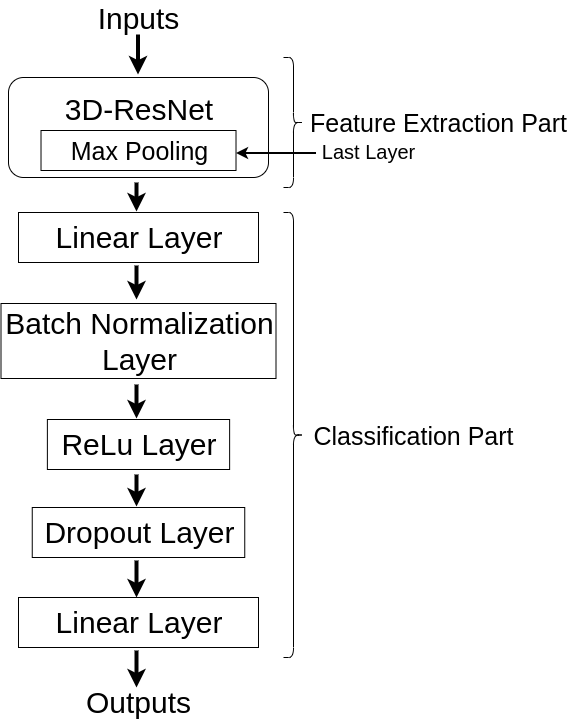
\includegraphics[width=65mm]{./fig/resnet3d_m_e.png}
        \label{fig:model24}
    }
    \caption{3D-ResNetチューニング後のモデル図}
\end{figure}

